\documentclass[11pt]{article}
\usepackage{color}
\usepackage{nth}
\usepackage{enumitem}
\usepackage{booktabs}
\usepackage{tabularx}
\usepackage{hyperref}
\usepackage[pdftex]{graphicx}
\usepackage{adjustbox}
\pagestyle{empty}
\setcounter{secnumdepth}{2}
\usepackage{float}
\usepackage{makeidx}
\makeindex
\usepackage{idxlayout}

\topmargin=0cm
\oddsidemargin=0cm
\textheight=22.0cm
\textwidth=17cm
\parindent=0cm
\parskip=0.15cm
\topskip=0truecm
\raggedbottom
\abovedisplayskip=3mm
\belowdisplayskip=3mm
\abovedisplayshortskip=0mm
\belowdisplayshortskip=2mm
\normalbaselineskip=12pt
\normalbaselines

% use case stuff
\newcounter{use case ID}

% environment slightly edited from https://tex.stackexchange.com/questions/10293/latex-template-for-use-cases
\newcommand\tabularhead[1]{
    \begin{table}[ht]
        \addtocounter{use case ID}{1}
        \caption{Use Case \arabic{use case ID} - #1}
        \vspace{0.2cm}
        \begin{tabular}{|p{0.2\linewidth}|p{0.70\linewidth}|}
            \hline
            \textbf{Action} & \textbf{#1} \\
            \hline}

        \newcommand\addrow[2]{#1 & #2\\ \hline}

            \newcommand\addmulrow[2]{ \begin{minipage}[t][][t]{2.5cm}#1\end{minipage}
                &\begin{minipage}[t][][t]{11cm}
                    \begin{enumerate}[itemsep=-1ex] #2   \end{enumerate}
                \end{minipage}\vfill\\ \hline}

            \newenvironment{usecase}{\tabularhead}
        {\hline\end{tabular}\end{table}}



        % cheaty non-functional requirement env

        \newcounter{req ID}
        \newcommand\tabularheadfsd[1]{
            \begin{table}[ht]
                \addtocounter{req ID}{1}
                \caption{Non-Functional Requirement \arabic{req ID} - #1}
                \vspace{0.2cm}
                \begin{tabular}{|p{0.2\linewidth}|p{0.70\linewidth}|}
                    \hline
                    \textbf{Action} & \textbf{#1} \\
                    \hline}

                \newenvironment{requirement}{\tabularheadfsd}
                {\hline\end{tabular}\end{table}}

                \begin{document}

                \vspace*{0.5in}
                \centerline{\bf\Large COMP 354}
                \centerline{\bf\Large Design document for 354TheStars}

                \vspace*{0.5in}
                \centerline{\bf\Large Group 5}

                \vspace*{0.5in}
                \centerline{\today}

                \begin{table}[htbp]
                    \caption{Group}
                    \begin{center}
                        \begin{tabular}{|r | c| c |}
                            \hline
                            Name & ID Number & Email \\
                            \hline
                            Morteza Ahmadi & 40038235 & morinob93@gmail.com \\
                            \hline
                            Mohd Tanvir & 40014010 & mohatanvir@hotmail.com \\
                            \hline
                            Arunraj Adlee & 40059206 & arunraj.adlee@hotmail.com \\
                            \hline
                            Dina Sadirmekova & 26321755 & dina.sadirmekova@gmail.com \\
                            \hline
                            Saima Syed & 40044790 & saima.syedb@gmail.com \\
                            \hline
                            Mehdi Skouri Saidi & 40057700 & mehdi879@hotmail.com \\
                            \hline
                            Trevor Lall & 40044047 & trevorlall95@gmail.com \\
                            \hline
                            Stefan John Bosco & 40057206 & johnboscostefan@gmail.com \\
                            \hline
                            Timothy Rodriguez & 40075447 & timmy\_258@hotmail.com \\
                            \hline
                            Lyonel Zamora & 27385986 & lyonelz516@gmail.com \\
                            \hline
                            Radhep Sabapathipillai & 40033092 & Radhep.Saba@gmail.com \\
                            \hline
                            Miguel Jimenez & 40022302 & migueleduardo298@hotmail.com\\
                            \hline
                        \end{tabular}
                    \end{center}
                \end{table}

                \begin{table}[htbp]
                    \caption{Revision history}
                    \begin{center}
                        \begin{tabular}{|r | c| c |}
                            \hline
                            Version & Date & Changes \\
                            \hline
                            1.0 & \nth{7} October 2019 & Completed requirements \\
                            \hline
                        \end{tabular}
                    \end{center}
                \end{table}


                \tableofcontents
\listoffigures
\clearpage
\listoftables

\clearpage




\section{Use Cases}
\subsection{Selling}

The use case diagram below represents the Selling functionality of the Online Shopping Website. A detailed description of each use case follows.

\begin{figure}[htbp]
    \centering
    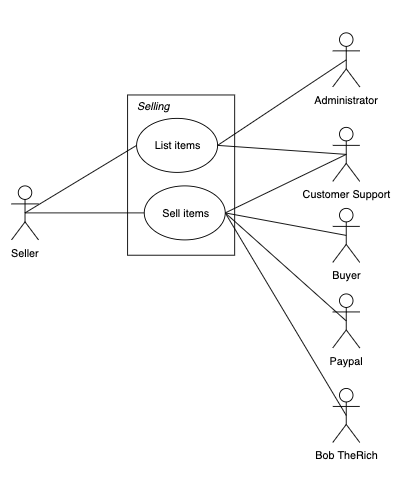
\includegraphics[width=0.5\textwidth]{Diagrams/Use_Case/ucd1.png}
    \caption{Use Case Diagram 1: Online Shopping Website - Selling }
    \label{fig:ucd1}
\end{figure}

\begin{usecase}{List items}
    \addrow{Case ID}{UC01}
    \addrow{Actors}{\textbf{Seller, Administrator, Customer Support}}
    \addrow{Summary}{\index{seller}Seller completes all the \index{information}information necessary to list an item and has the option to edit or delete it. The \index{administrator}Administrator can manage all the listings information. In case of any issues, the Customer Support can be contacted.}
    \addrow{Pre-Conditions}{The user is registered as a legitimate seller.}
    \addrow{\index{data}Data}{Product photo, \index{product}product description, price, stock count.}
    \addrow{Stimulus}{Seller pressed on Add Listing/Edit Listing/Delete Listing Button}
    \addmulrow{Response}{
            \item Add Listing/Edit Listing/Delete Listing dialogue appears.
            \item \index{seller}Seller fills out all the information.
            \item Listing added/edited/deleted successfully.
    }
    \addmulrow{Exceptions}{
            \item The required information is not filled out.
            \item The description is over the character limit (100 characters).
    }
    \addrow{Priority}{High}
    \addmulrow{Open Issues}{
            \item Should the \index{seller}Seller be able to preview the listing?
            \item What happens if the item is illegal?
            \item How do we check the quality of the image?
            \item How do we check if the seller is legitimate?
    }
\end{usecase}

\begin{usecase}{Sell items}
    \addrow{Case ID}{UC02}
    \addrow{Actors}{\textbf{Seller, Buyer, PayPal, Bob TheRich, Customer Support}}
    \addrow{Summary}{Seller accepts \index{payment}payment for the item from \index{buyer}Buyer and pays Bob TheRich the 8\% of the sale fee. The \index{seller}Seller can allow or disallow returns and set the time limit for returns. The Seller and Bob TheRich can access the sales history. In case of any issues, the Customer Support can be contacted.}
    \addrow{Pre-Conditions}{Seller, \index{buyer}Buyer, and Bob TheRich must have a valid \index{PayPal}PayPal account. }
    \addrow{\index{data}Data}{PayPal account \index{information}information, sales \index{data}data, returns option, time limit for returns, 8\% fee, shipped items}
    \addrow{Stimulus}{Buyer paid for item(s)}
    \addmulrow{Response}{
            \item \index{PayPal}PayPal transfers money from the \index{buyer}Buyer account to the Seller Account and sends a confirmation.
            \item \index{seller}Seller receives a sale notification by email.
            \item The sale appears in the Seller’s sales history.
            \item Bob TheRich invoices the Seller for 8\% of the sale.
            \item Seller pays Bob TheRich through PayPal.
            \item Seller marks item as shipped.
    }

    \addmulrow{Exceptions}{
            \item Confirmation from \index{PayPal}PayPal not received.
    }
    \addrow{Priority}{High}
    \addmulrow{Open Issues}{
            \item Should refunds be allowed? If yes, how should they be handled?
            \item What happens if the sale appears in the sales history but not in the shipped items history after a predetermined amount of time?
    }
\end{usecase}
\clearpage

\subsection{Buying}

The use case diagram below represents the Buying functionality of the Online Shopping Website. A detailed description of each use case follows.

\begin{figure}[htbp]
    \centering
    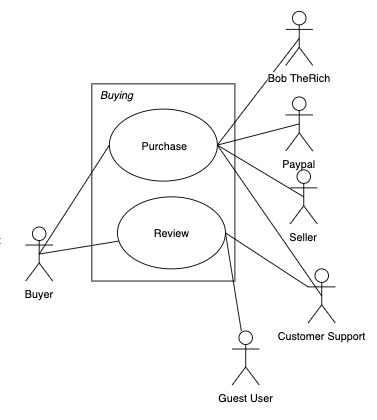
\includegraphics[width=0.5\textwidth]{Diagrams/Use_Case/ucd2.png}
    \caption{Use Case Diagram 2: Online Shopping Website - Buying }
    \label{fig:ucd2}
\end{figure}

\begin{usecase}{Purchase}
    \addrow{Case ID}{UC03}
    \addrow{Actors}{\textbf{Buyer, Seller, PayPal, Bob TheRich, Customer Support}}
    \addrow{Summary}{The Buyer views the shopping cart, has the option to modify it, and pays for it. In case of any issues, the Customer Support can be contacted.}
    \addmulrow{Pre-Conditions}{
        \item \index{buyer}Buyer is a \index{registered user}registered user.
        \item Buyer has a valid \index{PayPal}PayPal account.
        \item \index{seller}Seller contact is hidden.
    }
    \addrow{\index{data}Data}{Purchase photo, purchase description, purchase quantity, purchase price per item, total purchase price, taxes, shipping fee, shipping address, PayPal account, \index{receipt}receipt (Seller \index{information}information, Buyer information, purchase date, purchase details, purchase price, taxes)}
    \addrow{Stimulus}{Buyer presses the Checkout Button.}
    \addmulrow{Response}{
            \item \index{buyer}Buyer views the shopping cart information and can modify it.
            \item Buyer chooses the shipping option (standard or express).
            \item Buyer chooses the shipping address.
            \item Buyer pays the \index{seller}Seller for the purchase through \index{PayPal}PayPal.
            \item Buyer views the confirmation screen.
            \item Buyer receives a confirmation and \index{receipt}receipt by email.
            \item Order added to the purchase history.
    }
    \addmulrow{Exceptions}{
        \item Any of the required \index{information}information is missing or incorrect
        \item \index{buyer}Buyer exceeded the time limit to complete purchase
        \item Buyer abandons the cart
        \item Buyer did not receive a confirmation screen
    }
    \addrow{Priority}{High}
    \addmulrow{Open Issues}{
        \item What happens if the \index{buyer}Buyer is not allowed to purchase the \index{product}product legally?
    }

\end{usecase}

\begin{usecase}{Review}
    \addrow{Case ID}{UC04}
    \addrow{Actors}{\textbf{Buyer, Guest User, Customer Support}}
    \addrow{Summary}{\index{buyer}Buyer leaves a \index{review}review for a product previously purchased. In case of any issues, the Customer Support can be contacted.}
    \addrow{Pre-Conditions}{
        15 days must have passed since the \index{buyer}Buyer’s purchase of the \index{product}product being reviewed.
        }
    \addrow{\index{data}Data}{
Review text, \index{review}review photo, days since purchase, Buyer’s username, rating (out of 5 stars)
}
    \addrow{Stimulus}{Buyer clicks on the Add Review button}
    \addmulrow{Response}{
        \item \index{buyer}Buyer rates the \index{product}product
        \item Buyer adds \index{review}review text
        \item Buyer adds review photos (optional)
        \item Buyer posts the review
        \item Review appears on the product page for any \index{guest user}Guest User to view
    }
    \addmulrow{Exceptions}{
        \item 15 days haven’t passed since the purchase
        \item Buyer posted more than 5 photos per \index{review}review
        \item Review over the character limit (400 characters)
        \item Any of the required \index{information}information is missing
    }
    \addrow{Priority}{Medium}
    \addmulrow{Open Issues}{
        \item Should the \index{buyer}Buyer be able to preview the review?
        \item How do we handle offensive \index{review}reviews?
    }
\end{usecase}


\clearpage
\subsection{Login}

The use case diagram below represents the login functionality of the Online Shopping Website. A detailed description of each use case follows.

\begin{figure}[htbp]
    \centering
    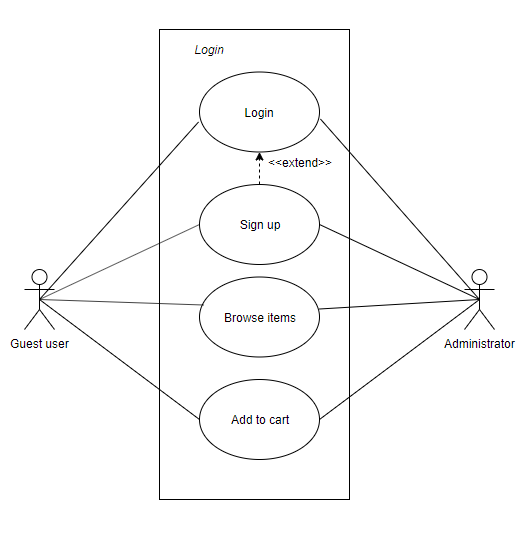
\includegraphics[width=0.5\textwidth]{Diagrams/Use_Case/ucd3.png}
    \caption{Use Case Diagram 3: Online Shopping Website - Login }
    \label{fig:ucd3}
\end{figure}

\begin{usecase}{Login}
    \addrow{Case ID}{UC05}
    \addrow{Actors}{\textbf{Guest user, Administrator}}
    \addrow{Summary}{Any \index{guest user}guest user can sign in to their account. Same goes for the \index{administrator}administrator.}
    \addmulrow{Pre-Conditions}{
        \item Must have an existing account
    }
    \addrow{\index{data}Data}{Username and password}
    \addrow{Stimulus}{\index{guest user}Guest user presses the login button.}
    \addmulrow{Response}{
            \item User will have the option to sell \index{product}products.
            \item User will have the option to buy products.
            \item User can browse and put items in his cart.
            \item \index{administrator}Administrator will have access to private \index{information}information.
            \item Administrator will be able to manege the website.
    }
    \addmulrow{Exceptions}{
        \item Username and/or password incorrect.
    }
    \addrow{Priority}{High}
    \addmulrow{Open Issues}{
        \item What if the \index{guest user}guest user forgets his/her password or username?
        \item Is there a limit of attempt for safety reason ?
    }

\end{usecase}

\begin{usecase}{Signup}
    \addrow{Case ID}{UC06}
    \addrow{Actors}{\textbf{Guest user, Administrator}}
    \addrow{Summary}{The \index{administrator}administrator and the \index{guest user}guest user should be able to create an account at any time.}
    \addrow{Pre-Conditions}{
       User has an email address.
        }
    \addrow{\index{data}Data}{
username, password, address, email, phone number
}
    \addrow{Stimulus}{\index{guest user}Guest user presses the sign up button}
    \addmulrow{Response}{
        \item user will have to fill out a formula.
        \item user will enter his/her personal \index{information}information.
        \item user will have access to more features.
    }
    \addmulrow{Exceptions}{
        \item User doesn't enter correct \index{information}information.
        \item Username taken/password weak.
    }
    \addrow{Priority}{High}
    \addmulrow{Open Issues}{
        \item What if the user already have an account and creates another one?
        \item How are we verifying that no two user have the same username?
        \item For security reasons,how are we handling weak passwords?
    }
\end{usecase}

\begin{usecase}{Browse item}
    \addrow{Case ID}{UC07}
    \addrow{Actors}{\textbf{Guest user, Administrator}}
    \addrow{Summary}{Both user can browse the items through the website and/or search for a specific item.}
    \addrow{Pre-Conditions}{
       None , anyone can browse.
        }
    \addrow{\index{data}Data}{
    item name, item description,item price}
    \addrow{Stimulus}{User write on the search bar}
    \addmulrow{Response}{
        \item the page will load all the items related.
        \item The page will display the pictures and prices of each item.
    }
    \addmulrow{Exceptions}{
        \item item not found (does not exist)
    }
    \addrow{Priority}{High}
    \addmulrow{Open Issues}{
        \item How are we handling spelling errors (ex;show suggestions) ?
    }
\end{usecase}



\begin{usecase}{Add to cart}
    \addrow{Case ID}{UC08}
    \addrow{Actors}{\textbf{Guest user, Administrator}}
    \addrow{Summary}{Whenever a user sees something that they like, they can put that item in their cart to eventually buy.}
    \addrow{Pre-Conditions}{
       Must be a \index{registered user}registered user.
        }
    \addrow{\index{data}Data}{
item picture, price of item, name of the \index{seller}seller,total price of all items chosen,quantity of each item chosen.}
    \addrow{Stimulus}{User click a button to add an item to his/her cart.}
    \addmulrow{Response}{
        \item The item will appear in the user's cart.
        \item The user will be able to go look at the cart.
        \item The user will be able to remove an item or continue adding.
    }
    \addmulrow{Exceptions}{
        \item Item is out of stock.
    }
    \addrow{Priority}{High}
    \addmulrow{Open Issues}{
        \item What happens to the cart if it contains items and the user exit the website?
    }
\end{usecase}
\clearpage
\section{Entity Relationship Diagram}
\begin{figure}[ht!]
    \centering
    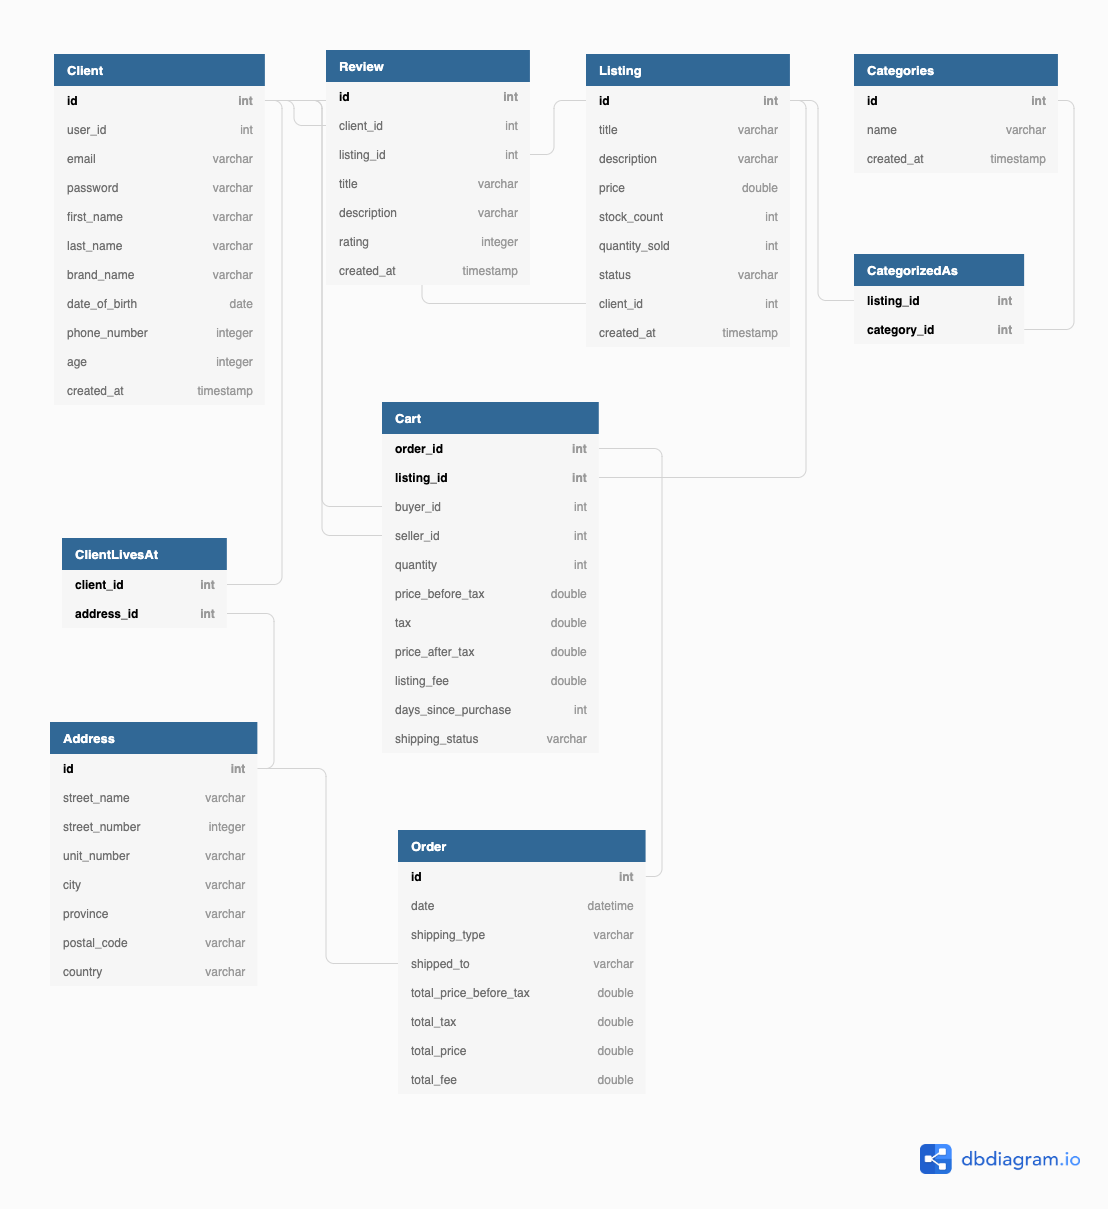
\includegraphics[width=0.9\textwidth]{Diagrams/ER/ER_Diagram_Typed.png} %I am not sure if this is the finalized picture.
    \caption{Entity Relationship Diagram With Their Associated Type}
    \label{fig:ER_Typed}
\end{figure}

\begin{figure}[ht!]
    \centering
    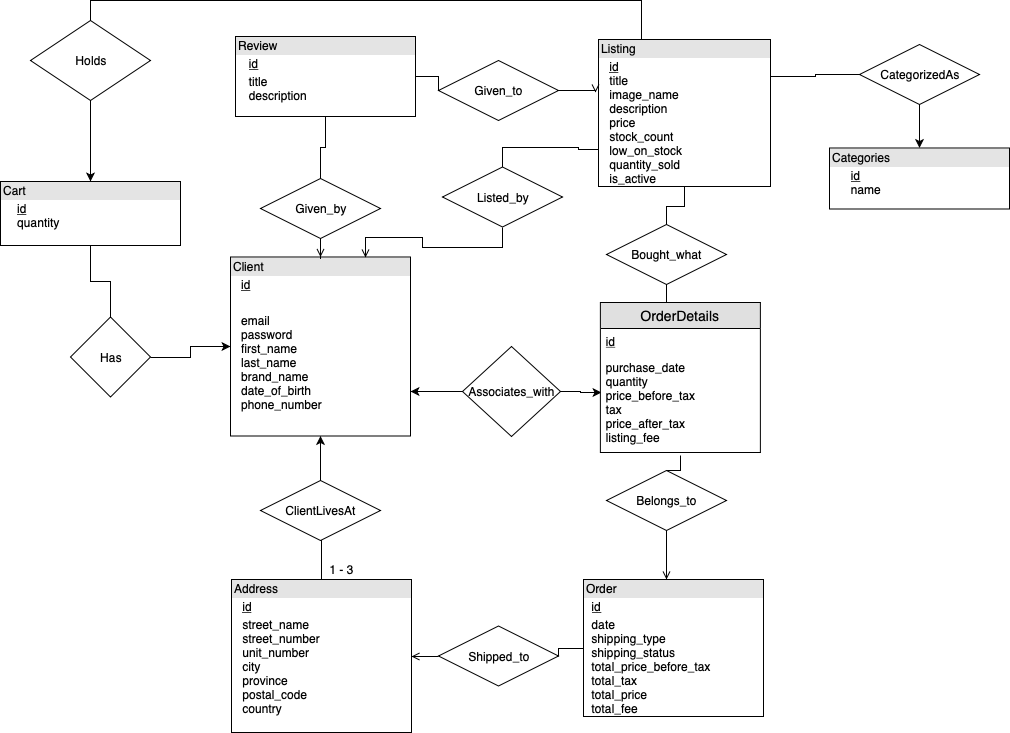
\includegraphics[width=0.9\textwidth]{Diagrams/ER/ER_Diagram.png}
    \caption{Entity Relationship Diagram}
    \label{fig:ER}
\end{figure}


\subsection{Description Of Each Entity}
\subsubsection{Client}
\subsubsection{Listings}
\subsubsection{Address}
\subsubsection{Order}
\subsubsection{Review}
\subsubsection{Order Details}
\subsubsection{Category}
\subsubsection{Cart}
\clearpage

\section{Class Diagram}
\begin{figure}[ht!]
    \centering
    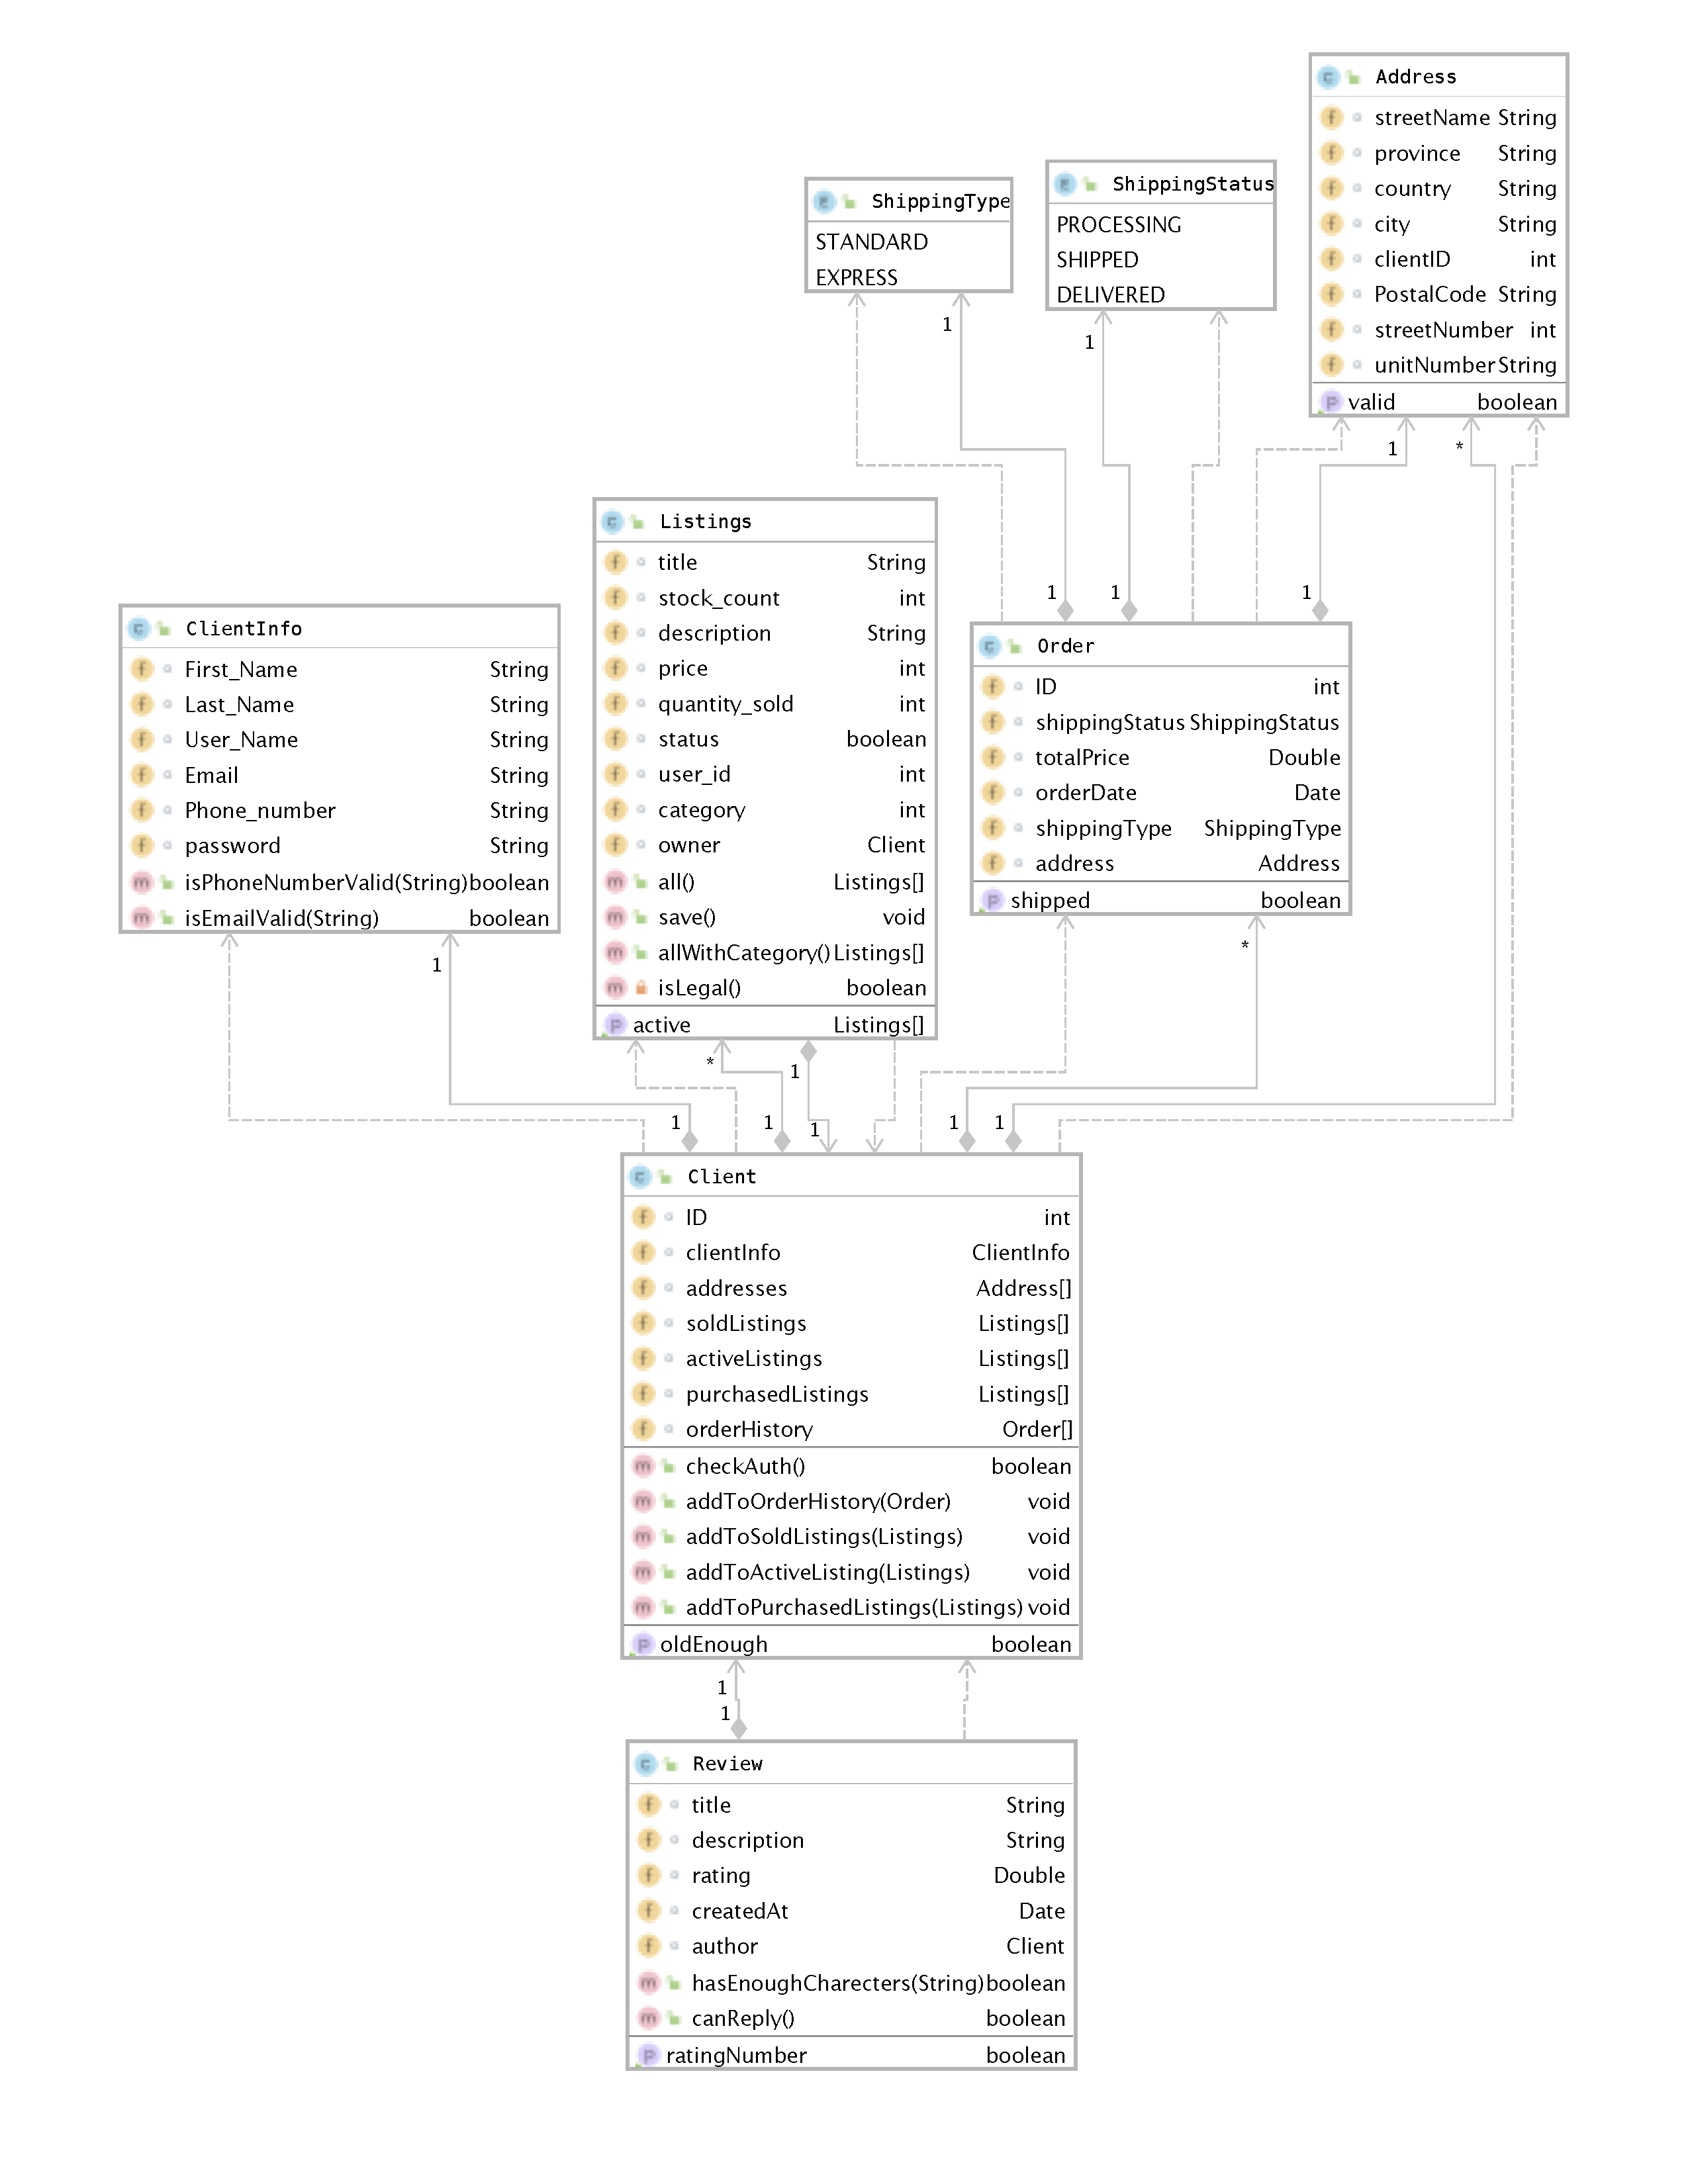
\includegraphics[width=0.8\textwidth]{Diagrams/Class/class_diagram.png} %I am not sure if this is the finalized picture.
    \caption{Class Diagram}
    \label{fig: Class diagram}
\end{figure}

\subsection{Description Of Class Diagram}
Write something about class diagram here!
\section{Sequence Diagram}
\begin{figure}[ht!]
    \centering
    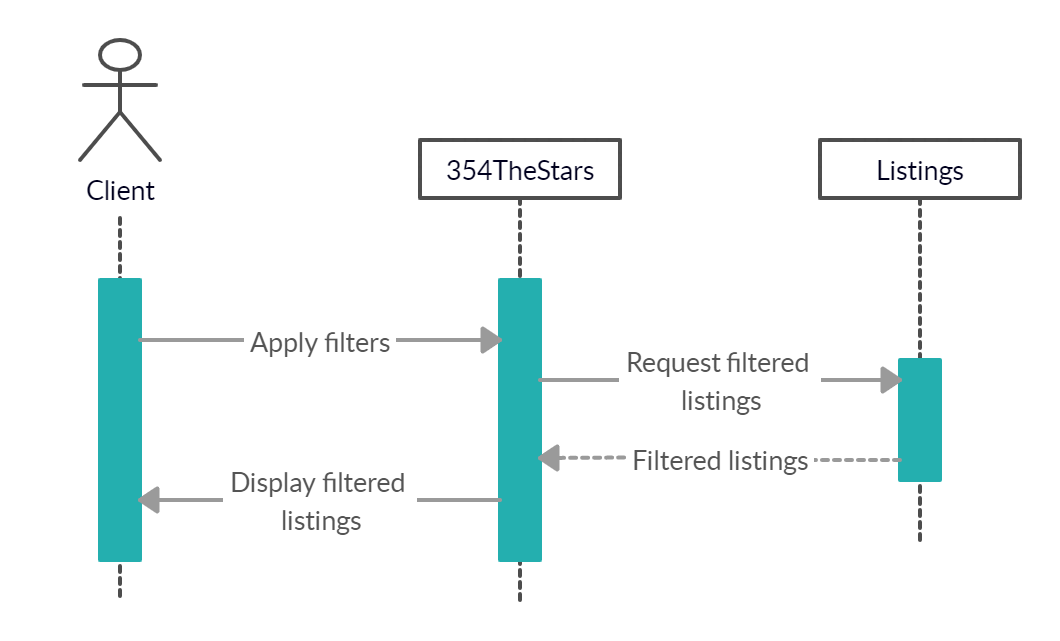
\includegraphics[width=0.6\textwidth,height=0.15\paperheight]{Diagrams/Sequence/Filter_Listings.jpg} 
    \caption{Filter Listings Results}
    \label{fig: Filter Listings Results}
\end{figure}
\begin{figure}[ht!]
    \centering
    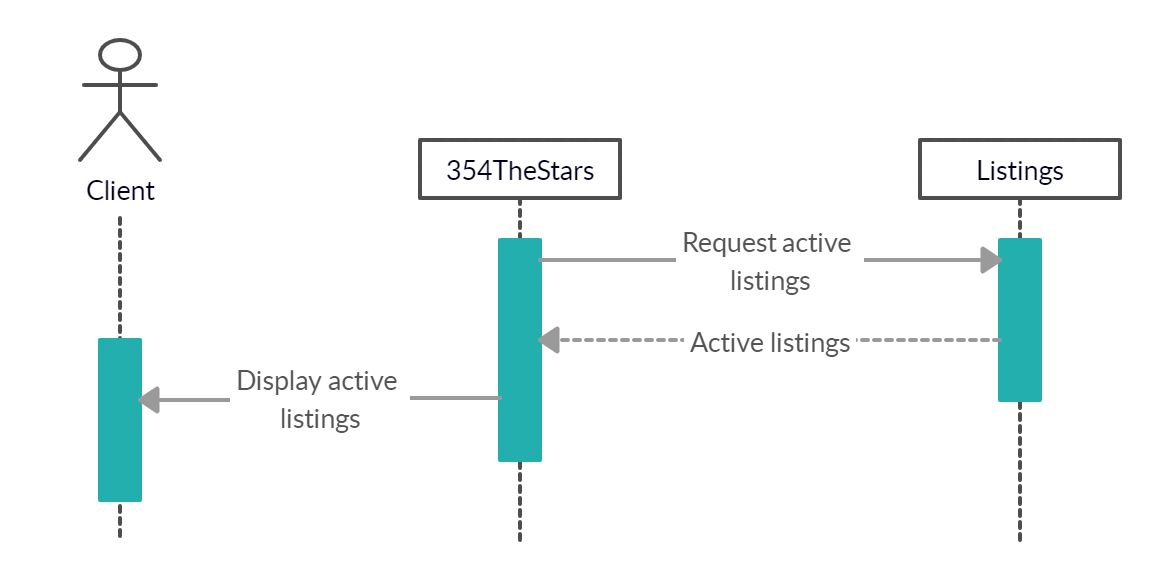
\includegraphics[width=0.6\textwidth,height=0.15\paperheight]{Diagrams/Sequence/Lists_of_Listings.jpg}
    \caption{Get Lists Of Listings}
    \label{fig: Get Lists Of Listings}
\end{figure}
\begin{figure}[ht!]
    \centering
    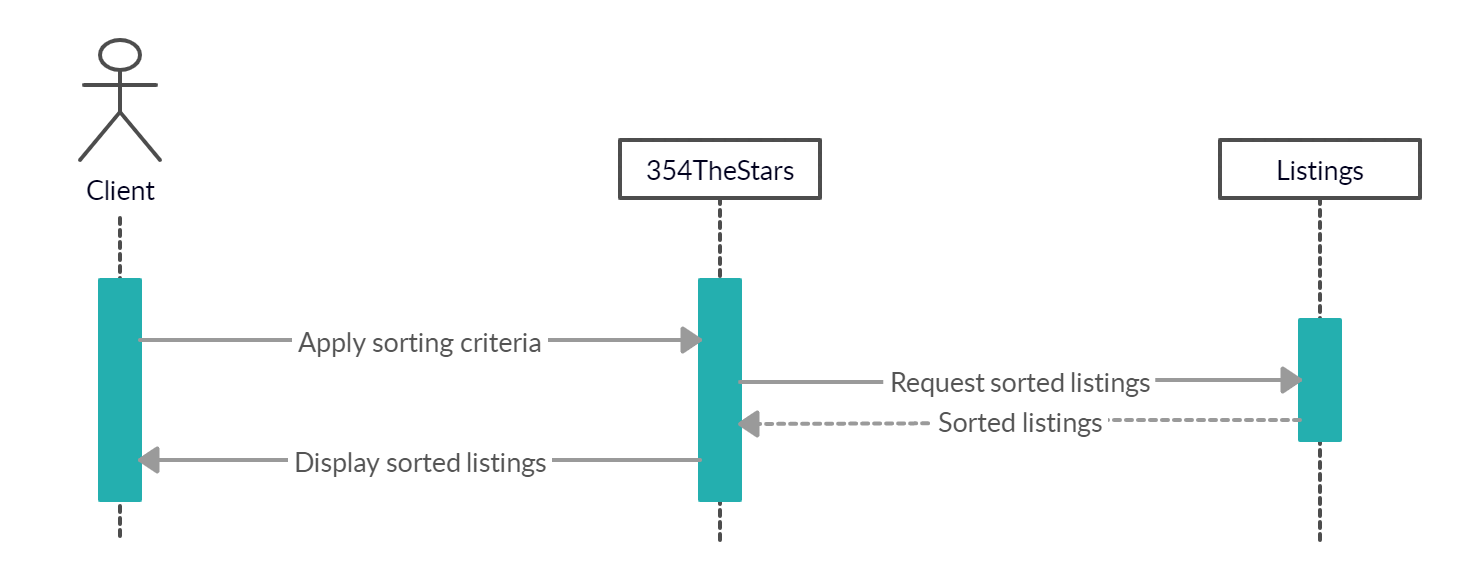
\includegraphics[width=0.6\textwidth,height=0.15\paperheight]{Diagrams/Sequence/Sort_Listings.jpg} 
    \caption{Sort Listings results}
    \label{fig: Sort Listings Results}
\end{figure}
\clearpage

\section{Architectural Diagram} 
\begin{figure}[ht!]
    \centering
    \includegraphics[width=\textwidth,height=0.6\paperheight]{Diagrams/Class/Architectural_diagram.png} 
    \caption{Architectural Diagram}
    \label{fig: Architectural Diagram}
\end{figure}

\section{External Interface}
\subsection{Home Page}
\begin{figure}[ht!]
    \centering
    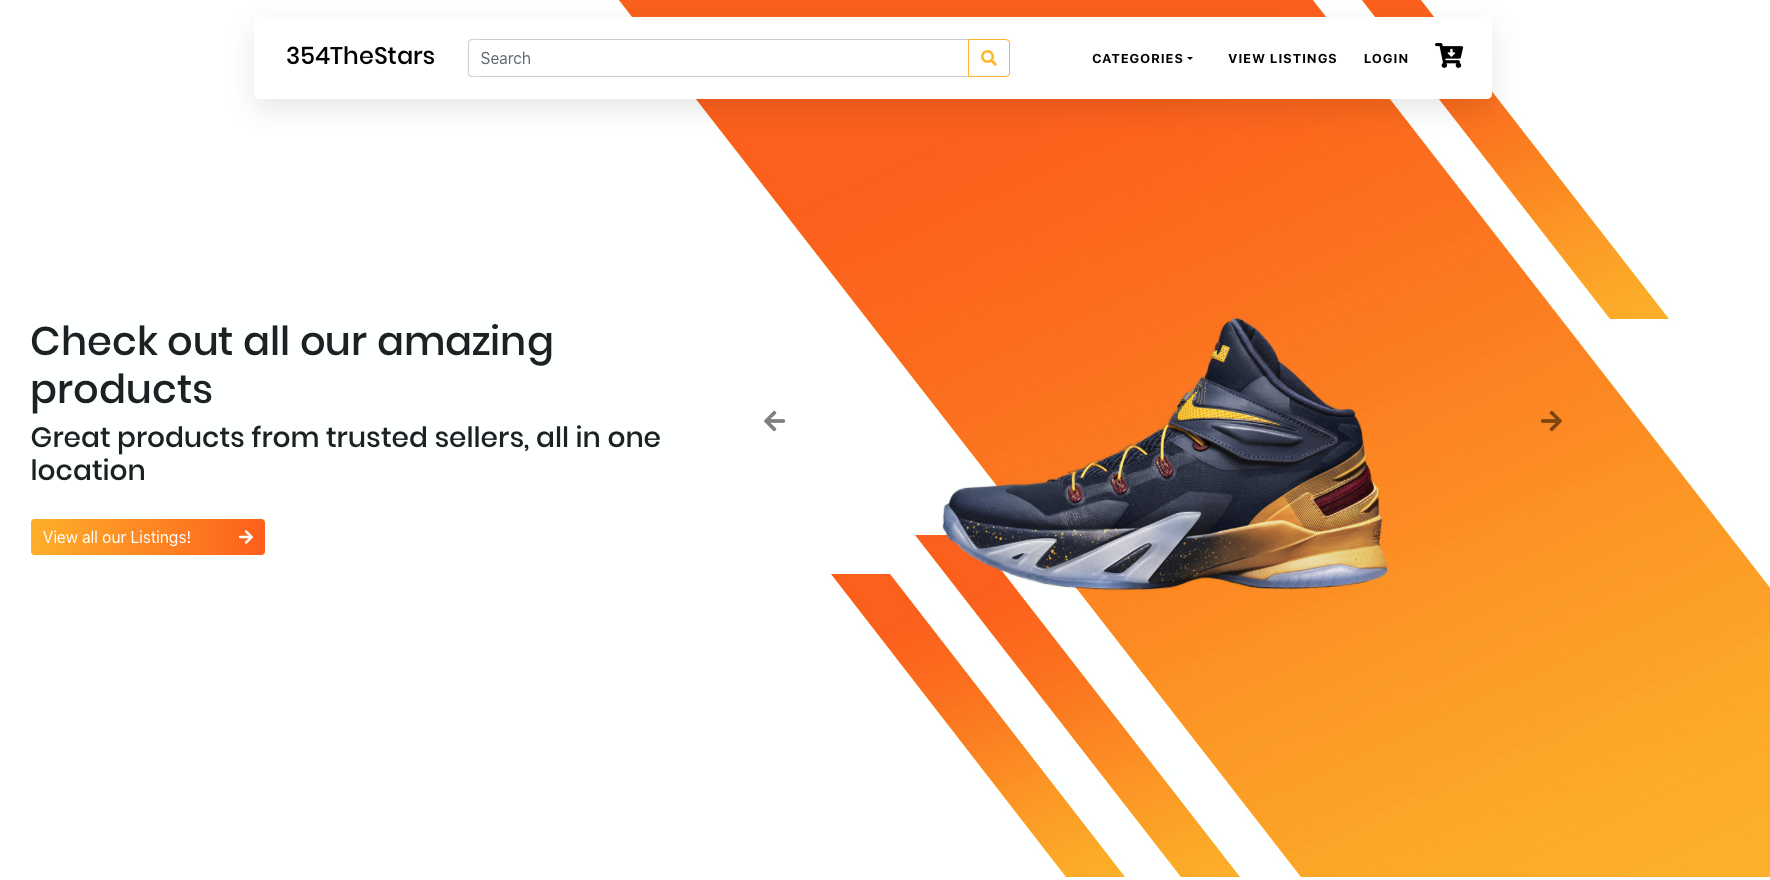
\includegraphics[width=\textwidth,height=0.4\paperheight]{Diagrams/External_Interfaces/Home_Page.png} %I am not sure if this is the finalized picture.
    \caption{Home Page}
    \label{fig: Home Page}
\end{figure}



\section{Conclusion}

With the continued evolution of technology, shoppers are moving away from retail
and embracing e-commerce sites. This is where 354TheStars comes in, which provides
a space for businesses and individuals to shop and/or sell all series of products
while they are home, at work, commuting, or from anywhere in the world as long
as they connect with a device and an internet connection. 354TheStars will bring
shoppers together as they review the products they have received with 354TheStars'
incredible shipping time, and share their experiences on the platform. With a
simple mission and a clear vision for what an e-commerce site should be, 354TheStars
is set to attract a great number of individuals and businesses.


\section{Index}

\printindex


\section{Reference}

\begin{itemize}
    \item User information: As our user and use-cases was based on feedback provided by our developers, our references lie mainly within our own team.
    \item Hakim Mellah's course COMP 354 content
    \item Ian Sommerville, Software Engineering. 10 Edition
    \item Roger S. Pressman, Software Engineering: a Practitioner's Approach, 7th edition
\end{itemize}
\end{document}
